% =============================================================
%  Gradient descent and the Gauss-Newton method
%  Computational Physics II (157219) - Unit 3
%  Compile with pdfLaTeX (two passes).
% =============================================================
\documentclass[aspectratio=169,10pt]{beamer}

\usepackage[utf8]{inputenc}
\usepackage{amsmath,amssymb}
\usepackage{booktabs}
\usepackage{array}
\usepackage{tikz}
\usepackage{pgfplots}
\pgfplotsset{compat=1.17}
\usepackage{listings}
\usepackage{tcolorbox}
\usetikzlibrary{arrows.meta,calc}

% ---------- Theme ----------
\usetheme[progressbar=frametitle,numbering=fraction,sectionpage=progressbar]{metropolis}
\usefonttheme[onlymath]{serif}   % classic LaTeX math typeface

\definecolor{tinta}{HTML}{14213D}
\definecolor{papel}{HTML}{FBF8F1}
\definecolor{arena}{HTML}{F2ECE0}
\definecolor{texto}{HTML}{2B3442}
\definecolor{cafe}{HTML}{A85A24}
\definecolor{azul}{HTML}{2F6FAD}
\definecolor{verde}{HTML}{1D7A5E}
\definecolor{gris}{HTML}{8A8F98}

\setbeamercolor{normal text}{fg=texto,bg=papel}
\setbeamercolor{background canvas}{bg=papel}
\setbeamercolor{palette primary}{fg=papel,bg=tinta}
\setbeamercolor{frametitle}{fg=papel,bg=tinta}
\setbeamercolor{alerted text}{fg=cafe}
\setbeamercolor{example text}{fg=azul}
\setbeamercolor{progress bar}{fg=cafe,bg=cafe!20}
\setbeamercolor{block title}{fg=tinta,bg=arena}
\setbeamercolor{block body}{fg=texto,bg=arena!45}
\setbeamercolor{block title alerted}{fg=papel,bg=cafe}
\setbeamercolor{block body alerted}{fg=texto,bg=cafe!8}
\setbeamertemplate{itemize item}{\color{cafe}\textbullet}
\setbeamertemplate{itemize subitem}{\color{gris}--}

% ---------- Helpers ----------
\newcommand{\grados}{\ensuremath{^\circ}}
\newtcolorbox{ecuacion}[1][]{colback=cafe!7,colframe=cafe,boxrule=0.6pt,arc=2pt,
  left=6pt,right=6pt,top=2pt,bottom=2pt,#1}
\newcommand{\fuente}[1]{\par\vfill{\scriptsize\color{gris}#1}}

\lstdefinestyle{py}{
  language=Python,
  basicstyle=\ttfamily\footnotesize\color{texto},
  keywordstyle=\color{cafe}\bfseries,
  commentstyle=\color{gris},
  stringstyle=\color{verde},
  backgroundcolor=\color{arena},
  frame=single, rulecolor=\color{arena},
  framesep=6pt, xleftmargin=6pt, xrightmargin=6pt,
  showstringspaces=false, columns=fullflexible, keepspaces=true,
  morekeywords={True,False,None},
}
\lstset{style=py}

% ---------- Title page ----------
\title{Gradient descent and the Gauss--Newton method}
\subtitle{Computational Physics II \;·\; Unit 3: Maxima and minima of functions}
\author{Sebastián}
\institute{Physics Program, Universidad de Pamplona}
\date{October 2026}

\begin{document}

\maketitle

\begin{frame}{Outline}
  \tableofcontents
\end{frame}

% =============================================================
\section{The problem}
% =============================================================

\begin{frame}{What does it mean to minimize?}
  Minimizing means finding the value of $x$ where $f(x)$ is as small as possible.
  \medskip

  In physics this comes up all the time:
  \begin{itemize}
    \item \textbf{Equilibrium.} A marble in a bowl settles where the potential energy is lowest.
    \item \textbf{Data fitting.} The curve that best describes a set of measurements is the one with the smallest error. This is the problem Gauss--Newton was designed for.
    \item \textbf{Neural networks.} Training one means minimizing a function of a huge number of variables, and it is done with variants of gradient descent.
  \end{itemize}
  \medskip

  Both methods we will see today work the same way at heart: start at some point and keep stepping downhill until you cannot go any lower.
  \note{I start with the general question. The three examples show this is not just a math topic. The second one is the one that matters most for us.}
\end{frame}

\begin{frame}{Why not just differentiate and set it to zero?}
  \begin{columns}[T]
    \begin{column}{0.45\textwidth}
      \centering
      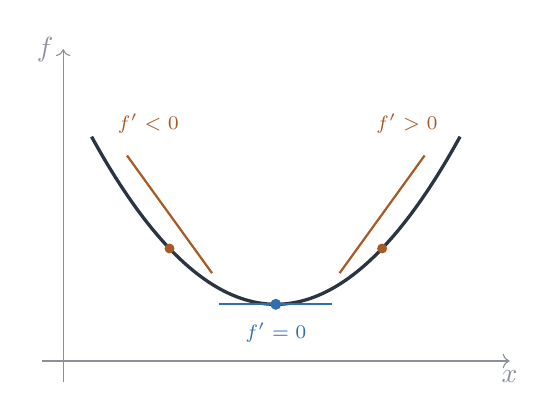
\begin{tikzpicture}[scale=0.9]
        \draw[->,gris] (-0.3,0) -- (6.3,0) node[below]{$x$};
        \draw[->,gris] (0,-0.3) -- (0,4.4) node[left]{$f$};
        \draw[very thick,texto,domain=0.4:5.6,smooth,samples=60] plot (\x,{0.35*(\x-3)^2+0.8});
        \draw[thick,cafe] (0.9,2.9) -- (2.1,1.24);
        \fill[cafe] (1.5,{0.35*(1.5-3)^2+0.8}) circle (2pt);
        \draw[thick,cafe] (3.9,1.24) -- (5.1,2.9);
        \fill[cafe] (4.5,{0.35*(4.5-3)^2+0.8}) circle (2pt);
        \draw[thick,azul] (2.2,0.8) -- (3.8,0.8);
        \fill[azul] (3,0.8) circle (2.2pt);
        \node[font=\scriptsize,cafe] at (1.2,3.35) {$f'<0$};
        \node[font=\scriptsize,cafe] at (4.85,3.35) {$f'>0$};
        \node[font=\scriptsize,azul] at (3,0.4) {$f'=0$};
      \end{tikzpicture}
    \end{column}
    \begin{column}{0.53\textwidth}
      At the bottom of the valley the tangent is horizontal: $f'(x^*) = 0$.
      \medskip

      The trouble is that we can rarely solve for $x$:
      \begin{itemize}
        \item Some equations have no closed-form solution, such as
          \[ 2x - e^{-x} = 0 . \]
        \item Sometimes $f$ comes from a simulation and there is no formula.
        \item With many variables it is not practical.
      \end{itemize}
      \medskip
      So we do what we did with Newton's method in Unit~2: start from an approximation and keep improving it.
    \end{column}
  \end{columns}
  \note{You already know the condition f prime equals zero from calculus. The key point is that in practice we cannot solve it directly, which is why we need iterative methods.}
\end{frame}

% =============================================================
\section{Gradient descent}
% =============================================================

\begin{frame}{The idea}
  Picture someone walking down a mountain in thick fog. They cannot see the valley; they can only feel which way the ground slopes, so they take a step downhill and repeat.
  \medskip

  In one variable this reads:
  \begin{ecuacion}
    \[
      x_{k+1} \;=\; x_k \;-\; \underbrace{\gamma}_{\text{step size}}\;\underbrace{f'(x_k)}_{\text{slope}}
    \]
  \end{ecuacion}
  \begin{itemize}
    \item The minus sign makes us always go downhill: if $f'(x_k)>0$ we move left, and if $f'(x_k)<0$, right.
    \item We choose $\gamma>0$ ourselves. In machine learning it is called the \emph{learning rate}.
    \item Where the slope is large, the step is large. Near the minimum $f'(x_k)\approx 0$, so the steps shrink on their own.
  \end{itemize}
  \note{This is the whole idea of the method. Stress the minus sign and the fact that we pick gamma.}
\end{frame}

\begin{frame}{A worked example}
  Take $f(x) = (x-3)^2 + 1$, with $f'(x) = 2(x-3)$ and minimum at $x^*=3$. We start at $x_0 = 0$ with $\gamma = 0.1$.
  \medskip

  \begin{columns}[T]
    \begin{column}{0.52\textwidth}
      \centering\small
      \begin{tabular}{ccccc}
        \toprule
        $k$ & $x_k$ & $f'(x_k)$ & $-\gamma f'(x_k)$ & $|x_k - 3|$ \\
        \midrule
        0 & 0     & $-6$     & $+0.6$   & 3 \\
        1 & 0.6   & $-4.8$   & $+0.48$  & 2.4 \\
        2 & 1.08  & $-3.84$  & $+0.384$ & 1.92 \\
        3 & 1.464 & $-3.072$ & $+0.307$ & 1.536 \\
        4 & 1.771 & $\cdots$ & $\cdots$ & 1.229 \\
        \bottomrule
      \end{tabular}
    \end{column}
    \begin{column}{0.46\textwidth}
      \centering
      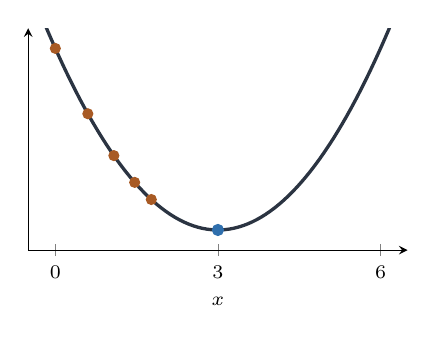
\begin{tikzpicture}
        \begin{axis}[width=6.4cm,height=4.4cm,axis lines=left,xmin=-0.5,xmax=6.5,ymin=0,ymax=11,
          xtick={0,3,6},ytick=\empty,xlabel={$x$},tick label style={font=\scriptsize},label style={font=\scriptsize}]
          \addplot[very thick,texto,domain=-0.3:6.3,samples=80] {(x-3)^2+1};
          \addplot[only marks,mark=*,mark size=1.8pt,cafe] coordinates {(0,10) (0.6,6.76) (1.08,4.6864) (1.464,3.359) (1.771,2.510)};
          \addplot[only marks,mark=*,mark size=2pt,azul] coordinates {(3,1)};
        \end{axis}
      \end{tikzpicture}
    \end{column}
  \end{columns}
  \medskip

  At each step the distance to the minimum is multiplied by $0.8$. It gets there, but slowly: after 20 steps we are still $0.035$ away.
  \note{Look at the last column: it is always multiplied by 0.8. That leads into the next slide.}
\end{frame}

\begin{frame}{The step size}
  Subtracting $3$ from both sides of the rule:
  \[
    x_{k+1} - 3 \;=\; (x_k - 3) - \gamma\cdot 2(x_k - 3) \;=\; (1 - 2\gamma)\,(x_k - 3).
  \]
  \begin{columns}[T]
    \begin{column}{0.5\textwidth}
      \centering\small
      \begin{tabular}{ccl}
        \toprule
        $\gamma$ & $1-2\gamma$ & What happens \\
        \midrule
        0.1 & $\phantom{-}0.8$ & goes down slowly \\
        0.5 & $\phantom{-}0$   & gets there in one step \\
        0.8 & $-0.6$ & zigzags, but closes in \\
        1   & $-1$   & oscillates between $0$ and $6$ \\
        1.1 & $-1.2$ & moves further away each time \\
        \bottomrule
      \end{tabular}
    \end{column}
    \begin{column}{0.47\textwidth}
      It converges if $|1-2\gamma|<1$, that is, if $0<\gamma<1$. The $2$ is the second derivative, so in general:
      \begin{ecuacion}
        \[ 0 \;<\; \gamma \;<\; \frac{2}{f''(x^*)} \]
      \end{ecuacion}
      In a very narrow valley (large curvature) we need short steps.
    \end{column}
  \end{columns}
  \medskip

  \alert{The weak spot of the method:} we have to choose $\gamma$, and the best value depends on the curvature, which the method does not use.
  \note{If there is time, show on the computer what happens when gamma changes.}
\end{frame}

% =============================================================
\section{Newton's method}
% =============================================================

\begin{frame}{Using the curvature}
  If we know $f''$, we can compute the step instead of guessing it. We replace $f$ by its Taylor parabola and jump to its vertex:
  \[
    f(x_k + h) \approx f(x_k) + f'(x_k)\,h + \tfrac{1}{2} f''(x_k)\,h^2
    \quad\Longrightarrow\quad
    f'(x_k) + f''(x_k)\,h = 0 .
  \]
  \begin{ecuacion}
    \[ x_{k+1} \;=\; x_k - \frac{f'(x_k)}{f''(x_k)} \]
  \end{ecuacion}
  \begin{itemize}
    \item It is the Newton--Raphson method from Unit~2 applied to $g(x)=f'(x)$, because we are looking for where $f'(x)=0$.
    \item If $f$ is a parabola, it gets there in one step. That is why $\gamma = 0.5 = 1/f''$ was the perfect step earlier.
  \end{itemize}
  \begin{alertblock}{About the name}
    Newman calls this formula the \emph{Gauss--Newton method}. In most optimization texts that name is reserved for least squares (Section~5).
  \end{alertblock}
  \note{Worth clarifying the name, since the professor will probably ask about the difference.}
\end{frame}

\begin{frame}{Newton versus gradient descent}
  Let us try a function that is not a parabola: $f(x)=\dfrac{x^4}{4}-x$, with minimum at $x^*=1$. Both start at $x_0 = 2$.
  \medskip

  \begin{columns}[T]
    \begin{column}{0.4\textwidth}
      \centering\small
      \begin{tabular}{ccc}
        \toprule
        $k$ & Newton & Gradient ($\gamma=0.2$) \\
        \midrule
        0 & 2      & 2 \\
        1 & 1.4167 & 0.6 \\
        2 & 1.1105 & 0.757 \\
        3 & 1.0106 & 0.870 \\
        4 & 1.0001 & 0.938 \\
        5 & 1.0000 & 0.973 \\
        \bottomrule
      \end{tabular}
    \end{column}
    \begin{column}{0.56\textwidth}
      \begin{itemize}
        \item With Newton the errors are $1,\ 0.42,\ 0.11,\ 0.011,\ 0.0001$: each one is roughly the square of the previous one (\textbf{quadratic} convergence).
        \item With gradient descent the error is multiplied by a fixed factor, about $0.4$ (\textbf{linear} convergence). The first step also overshoots the minimum.
        \item The price: Newton needs $f''$, and far from the minimum it can head to a maximum or diverge.
      \end{itemize}
    \end{column}
  \end{columns}
  \medskip

  \begin{ecuacion}
    Gradient descent is Newton's method with $1/f''(x_k)$ replaced by a constant $\gamma$.
  \end{ecuacion}
  \note{The first gradient step overshoots because the curvature is 12 at x=2 but only 3 at the minimum. No single fixed gamma works equally well everywhere.}
\end{frame}

% =============================================================
\section{Two variables}
% =============================================================

\begin{frame}{The gradient}
  \begin{columns}[T]
    \begin{column}{0.5\textwidth}
      Take $f(x,y) = x^2 + 10y^2$, a long, narrow valley. Differentiating with the other variable held fixed and putting both derivatives in a vector:
      \[ \nabla f = \left(\frac{\partial f}{\partial x},\, \frac{\partial f}{\partial y}\right) = (2x,\ 20y). \]
      For a small step $\Delta\mathbf r$:
      \[ \Delta f \approx \nabla f\cdot\Delta\mathbf r = |\nabla f|\,|\Delta\mathbf r|\cos\theta . \]
      \begin{itemize}
        \item $\theta = 0$: we climb as fast as possible.
        \item $\theta = 180\grados$: we descend as fast as possible.
        \item $\theta = 90\grados$: no change (level curve).
      \end{itemize}
    \end{column}
    \begin{column}{0.48\textwidth}
      \centering
      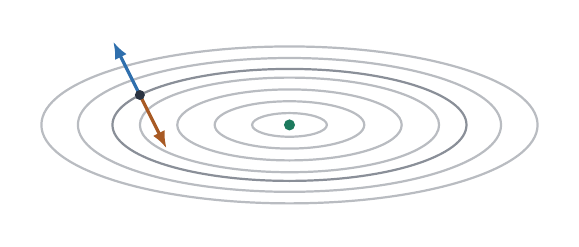
\begin{tikzpicture}[x=0.95cm,y=0.95cm]
        \clip (-3.5,-1.25) rectangle (3.5,1.3);
        \foreach \c in {0.25,1,2.25,4,8,11}{
          \draw[gris!60,thick] (0,0) ellipse ({sqrt(\c)} and {sqrt(\c/10)});
        }
        \draw[gris,thick] (0,0) ellipse ({sqrt(5.6)} and {sqrt(0.56)});
        \fill[verde] (0,0) circle (2pt);
        \draw[-{Latex[length=2.2mm]},very thick,azul] (-2,0.4) -- (-2.358,1.116);
        \draw[-{Latex[length=2.2mm]},very thick,cafe] (-2,0.4) -- (-1.642,-0.316);
        \fill[texto] (-2,0.4) circle (1.8pt);
      \end{tikzpicture}
      \smallskip

      {\scriptsize \textcolor{azul}{$\nabla f$}: steepest ascent \quad \textcolor{cafe}{$-\nabla f$}: steepest descent.\\ The gradient is perpendicular to the level curves.}
      \medskip

      \begin{ecuacion}
        \[ \mathbf r_{k+1} = \mathbf r_k - \gamma\,\nabla f(\mathbf r_k) \]
      \end{ecuacion}
    \end{column}
  \end{columns}
  \note{Notice that the orange arrow does not point at the minimum, the green dot. That explains the next slide.}
\end{frame}

\begin{frame}{The narrow valley problem}
  \centering
  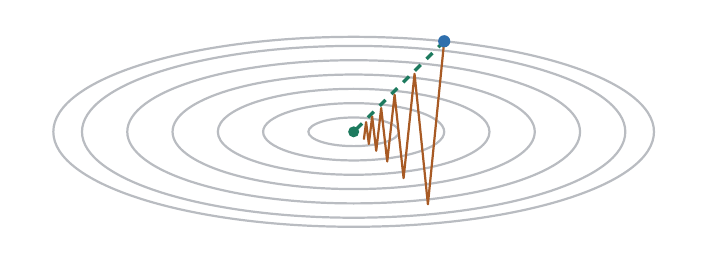
\begin{tikzpicture}[x=1.15cm,y=1.15cm]
    \begin{scope}
      \clip (-3.6,-1.15) rectangle (3.6,1.15);
      \foreach \c in {0.25,1,2.25,4,6.25,9,11}{
        \draw[gris!60,thick] (0,0) ellipse ({sqrt(\c)} and {sqrt(\c/10)});
      }
    \end{scope}
    \draw[very thick,verde,dashed] (1,1) -- (0,0);
    \draw[thick,cafe,line join=round] (1,1) -- (0.82,-0.8) -- (0.6724,0.64) -- (0.5514,-0.512) -- (0.4521,0.4096) -- (0.3707,-0.3277) -- (0.304,0.2621) -- (0.2493,-0.2097) -- (0.2044,0.1678) -- (0.1676,-0.1342) -- (0.1374,0.1074) -- (0.1127,-0.0859);
    \fill[azul] (1,1) circle (2.2pt);
    \fill[verde] (0,0) circle (2pt);
  \end{tikzpicture}

  {\scriptsize \textcolor{cafe}{Gradient descent with $\gamma = 0.09$} \quad \textcolor{verde}{Newton: a single step} \quad \textcolor{azul}{Start at $(1,1)$}}
  \raggedright
  \begin{columns}[T]
    \begin{column}{0.5\textwidth}
      \small
      Each direction has its own curvature: $2$ in $x$ and $20$ in $y$. With a single $\gamma$,
      \[ x_{k+1} = (1-2\gamma)\,x_k, \qquad y_{k+1} = (1-20\gamma)\,y_k . \]
      To keep $y$ from diverging we need $\gamma < 2/20 = 0.1$, and then $x$ barely moves.
    \end{column}
    \begin{column}{0.47\textwidth}
      \small
      With $\gamma = 0.09$: the factor is $0.82$ in $x$ and $-0.8$ in $y$, so $y$ flips sign at every step and the path bounces between the walls.
      \smallskip

      The ratio of the largest to the smallest curvature is the \textbf{condition number} (here, 10). The larger it is, the slower gradient descent becomes.
    \end{column}
  \end{columns}
  \note{Newton uses the curvature of each direction separately, so it reaches the center in one step. The Rosenbrock function, a standard test for these methods, has a condition number of about 2500.}
\end{frame}

% =============================================================
\section{The Gauss--Newton method}
% =============================================================

\begin{frame}{Fitting a model to data}
  \begin{columns}[T]
    \begin{column}{0.5\textwidth}
      \centering
      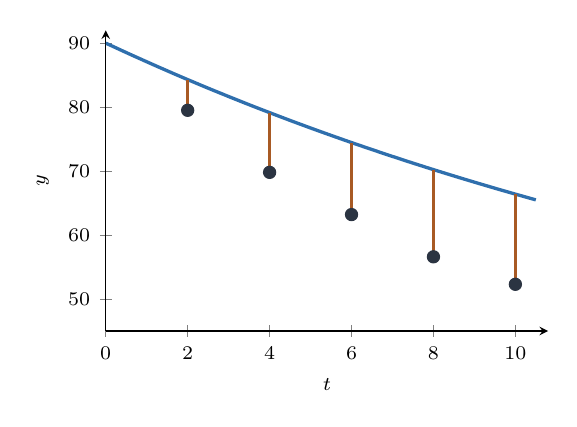
\begin{tikzpicture}
        \begin{axis}[width=7.2cm,height=5.4cm,axis lines=left,xmin=0,xmax=10.8,ymin=45,ymax=92,
          xlabel={$t$},ylabel={$y$},xtick={0,2,4,6,8,10},ytick={50,60,70,80,90},
          tick label style={font=\scriptsize},label style={font=\scriptsize}]
          \addplot[very thick,azul,domain=0:10.5,samples=60] {30+60*exp(-0.05*x)};
          \draw[very thick,cafe] (axis cs:2,79.5) -- (axis cs:2,84.29);
          \draw[very thick,cafe] (axis cs:4,69.8) -- (axis cs:4,79.12);
          \draw[very thick,cafe] (axis cs:6,63.2) -- (axis cs:6,74.45);
          \draw[very thick,cafe] (axis cs:8,56.6) -- (axis cs:8,70.22);
          \draw[very thick,cafe] (axis cs:10,52.3) -- (axis cs:10,66.39);
          \addplot[only marks,mark=*,mark size=2.2pt,texto] coordinates {(2,79.5) (4,69.8) (6,63.2) (8,56.6) (10,52.3)};
        \end{axis}
      \end{tikzpicture}

      {\scriptsize Dots: measurements. \textcolor{azul}{Curve}: model with a guessed parameter. \textcolor{cafe}{Segments}: residuals.}
    \end{column}
    \begin{column}{0.48\textwidth}
      We have data $(t_i, y_i)$ and a model $\phi(t;\beta)$ with an unknown parameter $\beta$.
      \medskip

      \textbf{Residual} (how far off the model is):
      \[ r_i(\beta) = \phi(t_i;\beta) - y_i \]
      \textbf{Sum of squares:}
      \[ S(\beta) = \sum_{i=1}^{m} r_i(\beta)^2 \]
      We square the residuals so that errors of opposite sign do not cancel out.
      \medskip

      \alert{Fitting = finding the $\beta$ that minimizes $S$.}
    \end{column}
  \end{columns}
  \note{If the measurement noise is Gaussian, minimizing S gives the most probable parameters; that was Gauss's justification in 1809. Minimizing S is minimizing a function of one variable, so we could use gradient descent or Newton, but Gauss found a shortcut.}
\end{frame}

\begin{frame}{The idea behind Gauss--Newton}
  \begin{columns}[T]
    \begin{column}{0.52\textwidth}
      \textbf{1. Sensitivity.} How much the model changes at each data point if we move $\beta$:
      \[ J_i = \frac{\partial \phi(t_i;\beta)}{\partial \beta} . \]
      \textbf{2. Linearize.} Near the current value we treat the model as a straight line:
      \[ r_i(\beta + \Delta) \approx r_i + J_i\,\Delta . \]
      \textbf{3. This leaves a parabola in $\Delta$:}
      \[ S(\Delta) \approx \sum_i \left(r_i + J_i\,\Delta\right)^2 . \]
    \end{column}
    \begin{column}{0.45\textwidth}
      \textbf{4. Its minimum.} Differentiate and set to zero:
      \[ \frac{dS}{d\Delta} = 2\sum_i \left(r_i + J_i\,\Delta\right)J_i = 0 \]
      \[ \sum_i J_i r_i + \Delta \sum_i J_i^2 = 0 \]
      \begin{ecuacion}
        \[ \Delta = -\,\frac{\displaystyle\sum_i J_i\, r_i}{\displaystyle\sum_i J_i^2} \]
      \end{ecuacion}
      Then $\beta \leftarrow \beta + \Delta$, and we repeat because the model is not really a straight line.
    \end{column}
  \end{columns}
  \note{In words: how far would I have to move the parameter so that, if the model were a straight line, the errors would cancel as well as possible? I move it that far and repeat.}
\end{frame}

\begin{frame}{Why is it called Gauss--Newton?}
  \begin{columns}[T]
    \begin{column}{0.55\textwidth}
      If we apply Newton to $S(\beta)$, the step would be $\Delta = -S'/S''$, with
      \begin{align*}
        S'  &= 2\sum_i J_i\, r_i, \\
        S'' &= 2\sum_i J_i^2 \;+\; \underbrace{2\sum_i r_i\,\frac{\partial^2 \phi_i}{\partial \beta^2}}_{\text{neglected}} .
      \end{align*}
      Dropping the last term:
      \[
        \Delta \approx -\frac{2\sum_i J_i r_i}{2\sum_i J_i^2} = -\frac{\sum_i J_i r_i}{\sum_i J_i^2},
      \]
      which is the same formula.
    \end{column}
    \begin{column}{0.42\textwidth}
      Gauss--Newton is Newton's method with the second derivative approximated using first derivatives only.
      \medskip

      \begin{block}{Why can we neglect it?}
        It is multiplied by the residuals, which are small when the model describes the data well.
      \end{block}
      \begin{block}{When does it fail?}
        When the starting value is far off, when the model is poor, or when two parameters do almost the same thing.
      \end{block}
    \end{column}
  \end{columns}
\end{frame}

\begin{frame}{More than one parameter}
  If the model has $n$ parameters $\boldsymbol\beta = (\beta_1,\dots,\beta_n)$, the sensitivity becomes an $m\times n$ matrix (one row per data point, one column per parameter):
  \[ J_{ij} = \frac{\partial \phi(t_i;\boldsymbol\beta)}{\partial \beta_j} . \]
  The same reasoning leads to the \emph{normal equations}:
  \begin{ecuacion}
    \[ \left(J^{\mathsf T} J\right)\boldsymbol\Delta \;=\; -\,J^{\mathsf T}\mathbf r \]
  \end{ecuacion}
  \begin{itemize}
    \item With a single parameter, $J^{\mathsf T}J = \sum_i J_i^2$ and $J^{\mathsf T}\mathbf r = \sum_i J_i r_i$: the previous formula.
    \item Each step requires solving an $n\times n$ linear system, using what we saw in Unit~1 (Gaussian elimination, LU).
  \end{itemize}
\end{frame}

% =============================================================
\section{Example: a cooling cup of coffee}
% =============================================================

\begin{frame}{Setting up the problem}
  \begin{columns}[T]
    \begin{column}{0.6\textwidth}
      We pour a coffee at $90\grados$C in a room at $30\grados$C and measure its temperature every two minutes. By Newton's law of cooling,
      \begin{ecuacion}
        \[ T(t) = T_a + (T_0 - T_a)\,e^{-k t} \]
      \end{ecuacion}
      with $T_a = 30\grados$C and $T_0 = 90\grados$C known. The only unknown is $k$ (in $\text{min}^{-1}$), which tells us how fast it loses heat.
      \medskip

      The sensitivity with respect to $k$ is
      \[ J_i = \frac{\partial T}{\partial k}(t_i) = -\,t_i\,(T_0 - T_a)\,e^{-k t_i} . \]
      We want the $k$ that minimizes $S(k) = \sum_i \big(T(t_i) - T_i\big)^2$.
    \end{column}
    \begin{column}{0.36\textwidth}
      \centering
      \begin{tabular}{cc}
        \toprule
        $t$ (min) & $T_i$ ($\grados$C) \\
        \midrule
        2  & 79.5 \\
        4  & 69.8 \\
        6  & 63.2 \\
        8  & 56.6 \\
        10 & 52.3 \\
        \bottomrule
      \end{tabular}
      \medskip

      {\scriptsize\color{gris}Simulated data with a little noise, made for this talk.}
    \end{column}
  \end{columns}
\end{frame}

\begin{frame}{First iteration by hand}
  We start from $k_0 = 0.05\ \text{min}^{-1}$.
  \medskip

  \centering\small
  \begin{tabular}{rrrrrrr}
    \toprule
    $t_i$ & $T_i$ & $T(t_i)$ & $r_i$ & $J_i$ & $J_i\,r_i$ & $J_i^2$ \\
    \midrule
    2  & 79.5 & 84.29 & 4.79  & $-108.6$ & $-520.1$     & 11\,790 \\
    4  & 69.8 & 79.12 & 9.32  & $-196.5$ & $-1\,832.1$  & 38\,610 \\
    6  & 63.2 & 74.45 & 11.25 & $-266.7$ & $-3\,000.1$  & 71\,126 \\
    8  & 56.6 & 70.22 & 13.62 & $-321.8$ & $-4\,382.0$  & 103\,525 \\
    10 & 52.3 & 66.39 & 14.09 & $-363.9$ & $-5\,128.3$  & 132\,437 \\
    \midrule
    \multicolumn{5}{r}{$\sum$} & $-14\,862.6$ & 357\,488 \\
    \bottomrule
  \end{tabular}
  \medskip

  \begin{ecuacion}
    \[ \Delta = -\frac{-14\,862.6}{357\,488} = 0.0416
       \qquad\Longrightarrow\qquad k_1 = 0.05 + 0.0416 = 0.0916\ \text{min}^{-1} \]
  \end{ecuacion}
  \raggedright
  All the residuals are positive: the model was cooling too slowly, so $k$ had to go up. That is why $\Delta$ comes out positive.
  \note{I can do this table on the board. Worth commenting on the sign of Delta at the end.}
\end{frame}

\begin{frame}{Results}
  \begin{columns}[T]
    \begin{column}{0.5\textwidth}
      \centering
      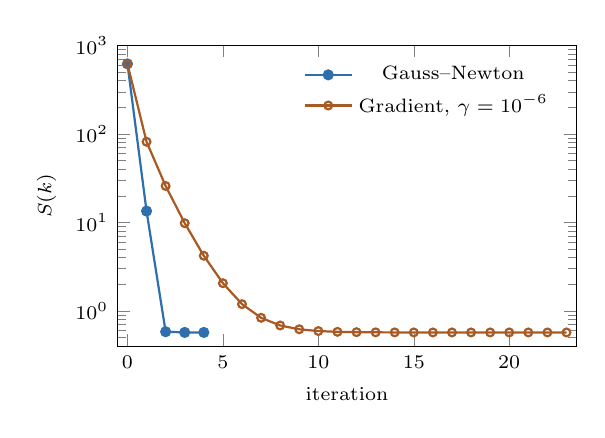
\begin{tikzpicture}
        \begin{semilogyaxis}[width=7.4cm,height=5.4cm,xmin=-0.5,xmax=23.5,ymin=0.4,ymax=1000,
          xlabel={iteration},ylabel={$S(k)$},
          tick label style={font=\scriptsize},label style={font=\scriptsize},
          legend style={font=\scriptsize,draw=none,fill=none},legend pos=north east]
          \addplot[thick,azul,mark=*,mark size=1.6pt] coordinates {(0,620.49) (1,13.453) (2,0.5829) (3,0.5718) (4,0.5718)};
          \addlegendentry{Gauss--Newton}
          \addplot[thick,cafe,mark=o,mark size=1.4pt] coordinates {(0,620.49) (1,81.71) (2,25.86) (3,9.815) (4,4.207) (5,2.060) (6,1.195) (7,0.8368) (8,0.6855) (9,0.6208) (10,0.593) (11,0.581) (12,0.5758) (13,0.5735) (14,0.5725) (15,0.5721) (16,0.5719) (17,0.5718) (18,0.5718) (19,0.5718) (20,0.5718) (21,0.5718) (22,0.5718) (23,0.5718)};
          \addlegendentry{Gradient, $\gamma=10^{-6}$}
        \end{semilogyaxis}
      \end{tikzpicture}
    \end{column}
    \begin{column}{0.48\textwidth}
      \centering
      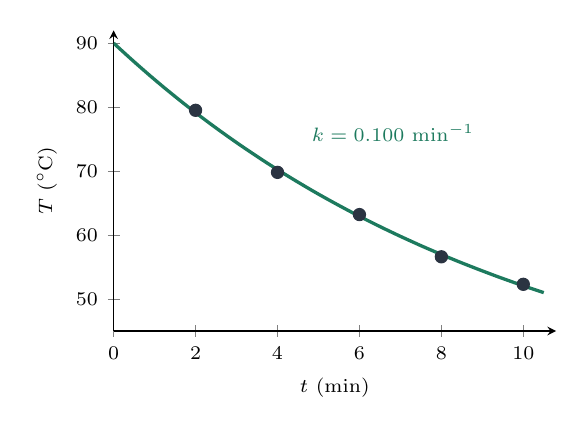
\begin{tikzpicture}
        \begin{axis}[width=7.2cm,height=5.4cm,axis lines=left,xmin=0,xmax=10.8,ymin=45,ymax=92,
          xlabel={$t$ (min)},ylabel={$T$ ($\grados$C)},xtick={0,2,4,6,8,10},ytick={50,60,70,80,90},
          tick label style={font=\scriptsize},label style={font=\scriptsize}]
          \addplot[very thick,verde,domain=0:10.5,samples=60] {30+60*exp(-0.1*x)};
          \addplot[only marks,mark=*,mark size=2.2pt,texto] coordinates {(2,79.5) (4,69.8) (6,63.2) (8,56.6) (10,52.3)};
          \node[font=\scriptsize,verde,anchor=west] at (axis cs:4.6,76) {$k = 0.100\ \text{min}^{-1}$};
        \end{axis}
      \end{tikzpicture}
    \end{column}
  \end{columns}
  \medskip

  Both reach $k \approx 0.100\ \text{min}^{-1}$: Gauss--Newton in 4 steps and gradient descent in 23. The sum of squares drops from 620 to 0.57; it does not reach zero because the data are noisy.
\end{frame}

\begin{frame}{How sensitive is gradient descent to $\gamma$?}
  \begin{columns}[T]
    \begin{column}{0.47\textwidth}
      \centering
      \begin{tabular}{cl}
        \toprule
        $\gamma$ & Result \\
        \midrule
        $1\times10^{-6}$ & 23 steps \\
        $3\times10^{-6}$ & 6 steps \\
        $5\times10^{-6}$ & 30 steps, oscillating \\
        $7\times10^{-6}$ & does not converge \\
        \bottomrule
      \end{tabular}
      \medskip

      \raggedright
      This matches what we saw in one variable, using $S''\approx 2\sum_i J_i^2 \approx 3.4\times10^{5}$:
      \begin{align*}
        \gamma_{\text{ideal}} &\approx \frac{1}{S''} \approx 2.9\times10^{-6}, \\[2pt]
        \gamma_{\text{max}}   &\approx \frac{2}{S''} \approx 5.9\times10^{-6}.
      \end{align*}
    \end{column}
    \begin{column}{0.49\textwidth}
      \begin{block}{Physical interpretation}
        With $k \approx 0.100\ \text{min}^{-1}$, the difference between the coffee and the room halves every
        \[ t_{1/2} = \frac{\ln 2}{k} \approx 6.9\ \text{min}. \]
        The final residuals are about $\pm 0.4\grados$C, on the order of the measurement noise.
      \end{block}
      Gauss--Newton does not need us to choose anything: it computes its own step.
    \end{column}
  \end{columns}
  \note{The question is: how could we have known in advance that gamma had to be around one millionth? Without knowing the curvature, there was no way.}
\end{frame}

\begin{frame}[fragile]{Python code (1/2): data and model}
\begin{columns}[T]
\begin{column}{0.66\textwidth}
\begin{lstlisting}
import numpy as np

# Simulated data (coffee in a room at 30 C)
t = np.array([2, 4, 6, 8, 10.0])              # min
T = np.array([79.5, 69.8, 63.2, 56.6, 52.3])  # C
T_amb, T0 = 30.0, 90.0                        # C

def model(k):  # Newton's law of cooling
    return T_amb + (T0 - T_amb)*np.exp(-k*t)

def residuals_and_J(k):
    r = model(k) - T                   # residuals
    J = -t*(T0 - T_amb)*np.exp(-k*t)   # dT/dk
    return r, J
\end{lstlisting}
\end{column}
\begin{column}{0.31\textwidth}
\small
\begin{itemize}
  \item \texttt{np.exp(-k*t)} evaluates all five times at once, with no loop.
  \item \texttt{r} holds the residuals $r_i$.
  \item \texttt{J} is the sensitivity $J_i = \partial T/\partial k$, worked out by hand.
  \item Both methods use these two functions.
\end{itemize}
\end{column}
\end{columns}
\end{frame}

\begin{frame}[fragile]{Python code (2/2): the two methods}
\begin{columns}[T]
\begin{column}{0.66\textwidth}
\begin{lstlisting}
# Gradient descent
k, gamma = 0.05, 1e-6
for i in range(100):
    r, J = residuals_and_J(k)
    step = -gamma * 2*np.sum(J*r)       # -gamma*dS/dk
    k += step
    if abs(step) < 1e-6: break
print("Gradient:     k =", round(k, 4), "in", i+1, "steps")

# Gauss-Newton
k = 0.05
for i in range(100):
    r, J = residuals_and_J(k)
    step = -np.sum(J*r) / np.sum(J**2)  # Gauss-Newton
    k += step
    if abs(step) < 1e-6: break
print("Gauss-Newton: k =", round(k, 4), "in", i+1, "steps")
\end{lstlisting}
\end{column}
\begin{column}{0.31\textwidth}
\small
Output:
\begin{lstlisting}[basicstyle=\ttfamily\fontsize{6.5}{8.5}\selectfont\color{texto},xleftmargin=0pt,xrightmargin=0pt,framesep=3pt]
Gradient:     k = 0.1 in 23 steps
Gauss-Newton: k = 0.1 in 4 steps
\end{lstlisting}
\begin{itemize}
  \item The two loops are identical except for the \texttt{step} line.
  \item They stop when the step is smaller than $10^{-6}$.
\end{itemize}
\end{column}
\end{columns}
\end{frame}

% =============================================================
\section{Wrapping up}
% =============================================================

\begin{frame}[fragile]{Levenberg--Marquardt: a blend of the two}
  Levenberg (1944) and Marquardt (1963) proposed adding a number $\mu \ge 0$ to the denominator:
  \begin{ecuacion}
    \[ \Delta = -\,\frac{\sum_i J_i\, r_i}{\sum_i J_i^2 + \mu} \]
  \end{ecuacion}
  \begin{itemize}
    \item If $\mu = 0$, it is Gauss--Newton.
    \item If $\mu$ is very large, $\Delta \approx -\dfrac{1}{\mu}\sum_i J_i r_i = -\dfrac{1}{2\mu}\,S'(\beta)$: a short gradient descent step with $\gamma = 1/(2\mu)$.
    \item If a step improves the fit, $\mu$ goes down; otherwise the step is rejected and $\mu$ goes up. Far from the solution it acts like gradient descent; close to it, like Gauss--Newton.
  \end{itemize}
  It is what SciPy's \texttt{curve\_fit} uses by default:
\begin{lstlisting}
from scipy.optimize import curve_fit
f = lambda t, k: 30 + 60*np.exp(-k*t)
k_opt, cov = curve_fit(f, t, T, p0=[0.05])   # k_opt = 0.1000 +/- 0.0009
\end{lstlisting}
\end{frame}

\begin{frame}{Comparison}
  \centering\small
  \renewcommand{\arraystretch}{1.25}
  \begin{tabular}{>{\raggedright\arraybackslash}p{2.0cm}>{\raggedright\arraybackslash}p{3.4cm}>{\raggedright\arraybackslash}p{3.4cm}>{\raggedright\arraybackslash}p{3.4cm}}
    \toprule
    & \textcolor{cafe}{\textbf{Gradient descent}} & \textbf{Newton} & \textcolor{azul}{\textbf{Gauss--Newton}} \\
    \midrule
    Problem & minimize any $f$ & minimize any $f$ & minimize a sum of squares \\
    Rule & $x - \gamma f'(x)$ & $x - f'(x)/f''(x)$ & $\beta - \sum J_i r_i \big/ \sum J_i^2$ \\
    Needs & $f'$ and a choice of $\gamma$ & $f'$ and $f''$ & first derivatives of the model \\
    Convergence & linear & quadratic (near the minimum) & nearly quadratic if the fit is good \\
    Weakness & choosing $\gamma$; zigzag in narrow valleys & expensive; unstable far from the minimum & unstable far away; fails with poor models \\
    \bottomrule
  \end{tabular}
\end{frame}

\begin{frame}{A bit of history}
  \begin{itemize}
    \item \textbf{1805.} Legendre publishes the method of least squares and gives it its name.
    \item \textbf{1809.} Gauss publishes it with a probabilistic justification (normally distributed errors) and claims he had been using it since 1795. Legendre disputed the priority.
    \item \textbf{1847.} Cauchy proposes the gradient method, also for orbit calculations.
    \item \textbf{1944 and 1963.} Levenberg and Marquardt propose the blend that bears their names.
  \end{itemize}
\end{frame}

\begin{frame}{Conclusions}
  \begin{itemize}
    \item Both methods move toward the minimum step by step. The difference is how much information they use to decide each step.
    \item Gradient descent only needs the first derivative. It is simple, but slow in narrow valleys, and its behavior depends heavily on $\gamma$.
    \item Gauss--Newton takes advantage of the sum-of-squares structure to approximate the curvature with first derivatives. That is why it converges so fast when the model describes the data well.
    \item In practice, data fitting uses Levenberg--Marquardt, which combines both.
  \end{itemize}
\end{frame}

\begin{frame}{References}
  \small
  \begin{itemize}
    \item M. Newman, \emph{Computational Physics}, CreateSpace, 2013. Section 6.4.
    \item S. C. Chapra and R. P. Canale, \emph{Numerical Methods for Engineers}, McGraw-Hill.
    \item J. Nocedal and S. J. Wright, \emph{Numerical Optimization}, 2nd ed., Springer, 2006. Chapters 3 and 10.
    \item W. H. Press \emph{et al.}, \emph{Numerical Recipes}, 3rd ed., Cambridge University Press, 2007. Section 15.5.
    \item S. M. Stigler, \emph{The History of Statistics}, Harvard University Press, 1986.
    \item K. Levenberg, ``A method for the solution of certain non-linear problems in least squares'', \emph{Quarterly of Applied Mathematics} 2 (1944) 164--168.
    \item D. W. Marquardt, ``An algorithm for least-squares estimation of nonlinear parameters'', \emph{Journal of the SIAM} 11 (1963) 431--441.
  \end{itemize}
\end{frame}

\begin{frame}[standout]
  Questions?
\end{frame}

\end{document}
